\documentclass[12pt, titlepage, a4paper]{article}
\usepackage[utf8]{inputenc}
\usepackage{changepage}
\usepackage{prftree}
\usepackage{amssymb}
\usepackage{amsmath}
\usepackage{enumitem} 
\usepackage{graphicx}
\usepackage{wrapfig}
\usepackage[spanish]{babel}
\usepackage{dirtytalk}
\usepackage{float}

\title{Introducción a la Inteligencia Artificial \\
Trabajo Práctico 1: Representación y Búsqueda en Espacio de Estados }
\author{Agunstin Fernandez Berge y Ramiro Gatto}
\date{14/04/2025}

\begin{document}
\maketitle

\section{Ejercicio 1}
Para implementar el algoritmo de DFS (Depth-First Search) utilizamos 
el algoritmo de búsqueda general, el cual es el siguiente:\\ 

\noindent Búsqueda General\\
\indent responde con \textbf{Solución} o \textbf{Falla}\\
\indent Lista-Nodo $\leftarrow$ Estado Inicial\\

\noindent bucle hacer\\
\indent si Lista-Nodo está vacía contestar \textbf{Falla}\\
\indent tomo NODO de Lista-Nodo\\
\indent si NODO es \textbf{meta} contestar con NODO\\
\indent Lista-Nodo $\leftarrow$ expansión NODO\\
\noindent FIN\\

En este caso, se colocan los NODOS generados al expandir, al comienzo de Lista-Nodos. 

Para lograr el comportamiento de \say{agregar NODOS al comienzo de Lista-Nodo} lo que  
decidimos utilizar fue una pila, la cual captura esa idea de agregar al inicio y sacar del inicio. 
Es decir, Lista-Nodos es una pila.\\

De esta forma, combinado el pseudo código y la pila es como implementamos 
el algoritmo de DFS. Luego al usar esta solución con el \textit{bigMaze} 
y con \textit{PositionSearchProblem} se obtiene:
\begin{verbatim}
    [SearchAgent] using function dfs
    [SearchAgent] using problem type PositionSearchProblem
    Path found with total cost of 210 in 0.02 seconds
    Search nodes expanded: 390
    Pacman emerges victorious! Score: 300
    Average Score: 300.0
    Scores:        300.0
    Win Rate:      1/1 (1.00)
    Record:        Win
\end{verbatim}

%Lo cual para nosotros en optimo

\section{Ejercicio 2}
Para la implementación de BFS (Breadth-First Search) también utilizamos el 
algoritmo de búsqueda general, solo que en este se colocan los NODOS generados 
al expandir al final de Lista-Nodos.\\

Para este comportamiento se utilizo una cola (normal), la cual permite 
agregar al final y sacar del inicio. Es decir, Lista-Nodos es una pila.
En este caso, nuevamente lo probamos con el \textit{bigMaze} y con \textit{PositionSearchProblem}
 obteniéndose:
\begin{verbatim}
    [SearchAgent] using function bfs
    [SearchAgent] using problem type PositionSearchProblem
    Path found with total cost of 210 in 0.02 seconds
    Search nodes expanded: 620
    Pacman emerges victorious! Score: 300
    Average Score: 300.0
    Scores:        300.0
    Win Rate:      1/1 (1.00)
    Record:        Win
\end{verbatim}


%Usando esta solucion se tiene lo siguiente ...
%Poner un analisis

\section{Ejercicio 3}
Para implementar UCS (Uniform Cost Search) nuevamente se utilizo el 
algoritmo de búsqueda general, solo que ahora al colocar los NODOS generados 
al expandir lo hacemos en base al costo del mismo. Agregando al inicio 
los de menor costo.\\

Para lograr esto se utilizan las colas de prioridad, siendo la prioridad 
el costo del nodo. Nuevamente probamos con el \textit{bigMaze} y con \textit{PositionSearchProblem}, 
teniéndose: 
\begin{verbatim}
    [SearchAgent] using function ucs
    [SearchAgent] using problem type PositionSearchProblem
    Path found with total cost of 210 in 0.02 seconds
    Search nodes expanded: 620
    Pacman emerges victorious! Score: 300
    Average Score: 300.0
    Scores:        300.0
    Win Rate:      1/1 (1.00)
    Record:        Win
\end{verbatim}

\section{Ejercicio 4}
\subsection{Búsqueda A*}
Recordemos que el A* utiliza una función $f(Nodo)$ de 
evaluación de la forma: $f(n) = g(n) + h(n)$ donde,
\begin{itemize}
    \item {g(n) = costo hasta llegar a n}
    \item {h(n) = costo estimado hasta la meta desde n}
    \item {f(n) = costo total de ruta pasando por n hasta la meta}
\end{itemize}

En este nuevamente utilizamos el algoritmo 
de búsqueda general 
en donde Lista-Nodos se ordena de
acuerdo al valor de $f(Nodo)$.\\

Para este caso utilizamos nuevamente las colas de prioridad, y ademas también nos 
fijamos si la heurística que se utiliza es consistente, antes de hacer la búsqueda.\\

Ahora, probamos con el \textit{bigMaze}, con \textit{PositionSearchProblem} y
 utilizando como heurística la \say{distancia de manhattan}.
teniéndose: 
\begin{verbatim}
    [SearchAgent] using function astar and heuristic manhattanHeuristic
    [SearchAgent] using problem type PositionSearchProblem
    Path found with total cost of 210 in 0.02 seconds
    Search nodes expanded: 549
    Pacman emerges victorious! Score: 300
    Average Score: 300.0
    Scores:        300.0
    Win Rate:      1/1 (1.00)
    Record:        Win
\end{verbatim}

En donde se puede observar que se corrobora la dicho en el enunciado, esto 
es que hay una diferencia de uno ~100 nodos expandidos con respecto a UCS.

\subsection{Laberinto openMaze}
En esta sección vamos a analizar las 4 forma de búsqueda que hicimos con 
el laberinto \textbf{openMaze}. El recorrido que hacen es el siguiente:

\begin{figure}[H]
    \centering
    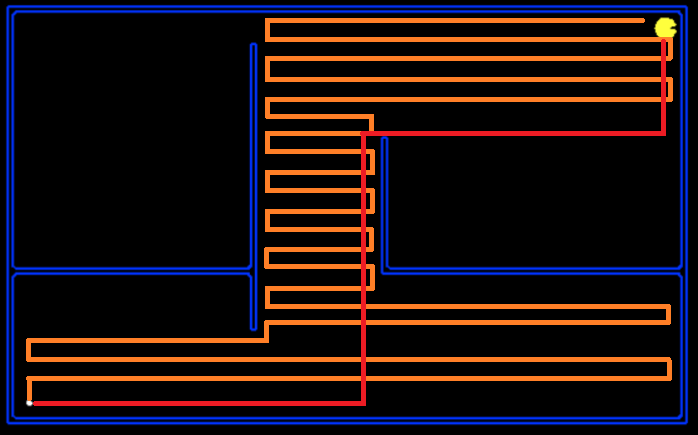
\includegraphics[width=.8\textwidth]{Imagenes/caminos.png}
    \caption{En naranja el camino del DFS, En rojo el camino del resto}
\end{figure}

Donde se tiene que todos menos el DFS siguen la misma ruta, pero 
exploran una cantidad de nodos distinto (535 en A*, 682 en UCS y en BFS, 576 en DFS). \\

A pesar de que A*, UCS y BFS expanden una cantidad distinta de nodos 
todos tienen el mismo puntaje (tardan lo mismo). Mas aun, a pesar de que DFS es uno de los que 
menos nodos expande este es el de peor puntaje (mas lento).


%%A*
%%Path found with total cost of 54 in 0.03 seconds
%%Search nodes expanded: 535
%%Pacman emerges victorious! Score: 456
%%
%%UCS
%%Path found with total cost of 54 in 0.02 seconds
%%Search nodes expanded: 682
%%Pacman emerges victorious! Score: 456
%%
%%DFS
%%Path found with total cost of 298 in 0.02 seconds
%%Search nodes expanded: 576
%%Pacman emerges victorious! Score: 212
%%
%%BFS
%%Path found with total cost of 54 in 0.02 seconds
%%Search nodes expanded: 682
%%Pacman emerges victorious! Score: 456

\section{Ejercicio 5}
\subsection{cornersProblems}
En este ejercicio tenemos que elegir una forma de representar el estado de 
tal forma que detecte si las 4 esquinas del laberinto fueron alanzadas. La 
forma que elegimos fue tomar al estado como: \textbf{(Posición actual, (Bool, Bool, Bool, Bool))}.\\

\noindent Es decir, el estado es una tupla cuyas componentes son:
\begin{itemize}
    \item {La posición actual.}
    \item {Una cuádrupla de Bool, cada uno representa una esquina del tablero en este orden: (1, 1), (1, top), (right, 1), (right, top). Al 
        principio estan todas en False.}
\end{itemize}

De esta forma cuando se llega a una esquina se cambia el False correspondiente por 
un True. Para ver si se alcanzaron todas las esquinas se hace un And generalizado 
entre todas las componentes de la cuádrupla.\\

\subsection{Posibles heurísticas}
Para el tema de las heurística se pensaron unas cuantas, y para ver si es admisible hay que 
tener en cuenta que la heurística no debe sobrestimar. La primera que se pensó fue
\begin{center}
    Distancia de manhattan a la esquina no visitada mas cercana\\ 
    
    +\\ 
    
    Distancia de manhattan a la esquina no visitada mas cercana a la encontrada anteriormente 
\end{center}

De esta forma se disminuye considerablemente los nodos explorados 
pero tiene un problema, no es consistente, pero podría ser admisible por estar usando la 
distancia de manhattan.\\

La siguiente forma fue considerar la cantidad de esquinas no visitadas.
 Esta es aparentemente consistente, por lo que es admisible. Pero con la desventaja de que 
 la cantidad de nodos explorados es alta.\\ 

Otra que se pensó fue, distancia de manhattan a la esquina no visitada mas cercan. 
Esta expande mas nodos, pero resulto ser inconsistente. Aunque podria llegar al ser consistente por la 
distancia de manhattan.\\

También se pendo reutilizar el primer método pero modificandolo para volverlo consistente y 
por consecuente que sea admisible, surgiendo:
\begin{itemize}
    \item {Esta vez usando la distancia euclidea. Se obtiene un resultados similares,
            sigue sin ser consistente pero la diferencia entre h(n) y c(n,n')+h(n') es cada vez menor.
            Peor aun, por la forma en la que se mueve el pacaman (arriba, abajo, izquierda, derecha) 
            no seria admisible.}
    \item {Usar la norma infinito: De esta forma seria consistente, por lo que es admisible. 
            Pero expande muchísimos menos nodos.}
\end{itemize}

\noindent La ultima heurística que pensamos fue:
\begin{center}
    Revisar todos los ordenes posibles para visitar las esquinas 
    y calcular el menor recorrido total entre todos los ordenes. 
\end{center}

Puede sonar prohibitivamente lento (de hecho, la complejidad es O(n!) por cada calculo de la heurística), 
pero como solo son 4 pastillas hay que revisar como mucho 4! = 24 posibles ordenes. Se pueden precomputar 
algunos resultados para bajar la complejidad a O(1). 
Es aparentemente admisible y consistente, y ademas disminuye muchísimo la cantidad de nodos explorados, 
(menos de 800 nodos explorados en mediumCorners (expande 741 nodos)).

\section{Ejercicio 6}
La heurística elegida para el es aquella que corresponde a la
resolución del problema de comer las pastillas en las esquinas cuando no hay
paredes en el laberinto.\\

$h(n)= \text{numero minimo de pasos para alcanzar las 4 esquinas si no hay paredes}$\\

La heurística es admisible, ya que el numero de pasos para obtener las pastillas
en un laberinto vació no puede disminuir si se colocan paredes, por lo que la
heurística no sobrestima el costo de la solución.\\

\noindent Veamos como seria el caso general\\

Este algoritmo para encontrar la distancia puede usarse para resolver el caso
donde la posición inicial S no esta en las esquinas.

\begin{verbatim}
        +-------------------+
        |A                 B|
        |                   |
        |         S         |
        |                   |
        |C                 D|
        +-------------------+
\end{verbatim}


En este caso cualquier ruta de menor coste tiene que empezar por alguno de los
siguieres casos:
\begin{enumerate}
    \item {S $\rightarrow$ A $\rightarrow$ ...}
    \item {S $\rightarrow$ B $\rightarrow$ ...}
    \item {S $\rightarrow$ C $\rightarrow$ ...}
    \item {S $\rightarrow$ D $\rightarrow$ ...}
\end{enumerate}

Todos los casos continúan en un escenario donde hay que llegar desde una esquina
del tablero a todas las demás, por lo que se puede usar el algoritmo greedy 
para resolver estos casos.\\

Asi, un candidato a solución puede obtenerse calculando la distancia desde el punto
inicial S a todas las esquinas y luego calcular la distancia faltante usando
el algoritmo greedy. La solución del problema general consiste en el mínimo de
todos los candidatos a solución(que son 4, por lo que computar la solución no
es muy costoso).

\section{Ejercicio 7}


\end{document}